\def\year{2020}\relax
\documentclass[letterpaper]{article} 
\usepackage{../aaai22}  
\usepackage{times}  
\usepackage{helvet} 
\usepackage{courier}  
\usepackage[hyphens]{url}  
\usepackage{amsthm}
\usepackage{amsmath,amssymb}\usepackage{graphicx} 
\urlstyle{rm} 
\def\UrlFont{\rm}  
\usepackage{graphicx}  
\frenchspacing  
\setlength{\pdfpagewidth}{8.5in}  
\setlength{\pdfpageheight}{11in}  
\newcommand{\citename}[1]{\citeauthor{#1}~\shortcite{#1}}
\DeclareMathOperator{\argmax}{argmax}
\DeclareMathOperator{\argmin}{argmin}



\setcounter{secnumdepth}{2}

\setlength\titlebox{2.5in} 
\title{Interpretable Models of Human Interaction in Immersive Simulation Settings}
 \author{Paper ID 134 (this is the rejected AAAI paper)}


\newcount\Comments  
\Comments=1

\usepackage{xcolor}
\newcommand{\kibitz}[2]{\ifnum\Comments=1{\textcolor{#1}{#2}}\fi}
\newcommand{\nh}[1]{\kibitz{blue}{[NH:#1]}}
\newcommand{\kg}[1]{\kibitz{red}{[KG:#1]}}
\newcommand{\bjg}[1]{\kibitz{purple}{[BG:#1]}}

 \begin{document}






























































































































































\section{User Study}
\label{sec:interpretability_results}













All participants received a detailed tutorial about CW and the study, as well as a pre-study comprehension quiz\footnote{Tutorial pdf slides are available in the supplementary material.}. Mturk workers were paid a base rate of $\$0.25$ for participating and a bonus structure of $\$0.1$ for each correct response.






\begin{figure}[t]


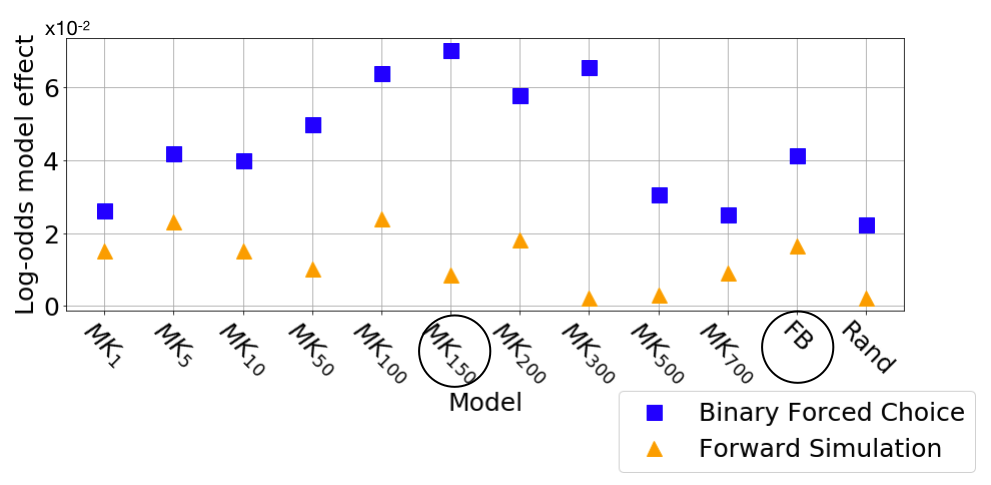
\includegraphics[width=.48\textwidth]{../combined_res_data_all.png}
\caption{Effect of each model on the log-odds of a test evaluator selecting the correct response (controlling for the test evaluator, the experiment trial, log file and ordering effects).}
\label{fig:essil_test_results}
\end{figure}


We first describe results in terms of accuracy (the percent of correctly labelled test instances).
The top performing model was $MK_{200}$ with an accuracy of $83\%$ on the Forward Simulation  test and $MK_{100}$  with an accuracy of $82\%$ on the Binary Forced Choice test.
The random baseline model performed consistently poorly with an average accuracy of $53\%$ on both tests.
The fully Bayesian model achieved an accuracy of $72\%$ and $70\%$ respectively on the two tests.

To control for ordering effects, chosen time periods, data instance used, and effects of individual participants, we applied an L2 regularized logistic regression for predicting  the user specific success on the experiment trial, shown  in  Figure~\ref{fig:essil_test_results}. The y-axis presents the improvement in log-odds that a model has on the expected response accuracy (higher is better).
As shown by the figure,  the Forward Simulation shows a high variance with no clear maximum. In contrast, the Binary Forced Choice test has a clear maximum in the region of $MK_{100}$ and $MK_{150}$.

From both Figures~\ref{fig:dic_waic_scores} and~\ref{fig:essil_test_results} we can infer the following four conclusions.
First, all of the models ($MK_{1},\ldots,MK_{700}, FB$) outperform the random baseline: participants are more likely to select the correct response from any of these models. This result suggests that periods of stable dynamics  exist in the data and that it is possible to construct models, which describe these dynamics, that are interpretable to people.

Second, the Binary Forced Choice test is a preferable measure for interpretablity   to the Forward Simulation test. Figure~\ref{fig:essil_test_results} shows that the Binary Forced Choice test exhibits a clear peak (around $MK_{100}$ and $MK_{150}$) where interpretability of the model is maximized.
These models also maximized the  raw accuracy on the Binary Forced Choice test.

On the other hand, the Forward Simulation test has a greater variance across models and across data instances.
Two possible causes for this higher variance are: (1) there is more room for error in the Forward Simulation test (5 choices vs. 2 choices in Binary Forced Choice); (2) sampling a single image to represent a period (as in Forward Simulation) presents less information to the user than sampling 4 images (as in Binary Forced Choice).

Third, the best $\kappa$ settings vary for different tests and information criteria.
Model interpretability grows steadily as the value of $\kappa$ increases, with $MK_{100}$ and $MK_{150}$ being the optimal models, and then proceeds to decrease steadily.
These models are not consistent with the model $MK_5$ that optimized the information criteria.
Note that higher $\kappa$ values are ``sticky'' - they  bias the model towards longer periods, which condense too many activities to make sense to people.
On the other end of the spectrum, lower $\kappa$ values allow for shorter periods that capture too much of the noise in the system.
In contrast, the $\kappa$ value for  models $MK_{100}$ and $MK_{150}$
represent a ``sweet spot" in between these two extremes.


Finally, the fully Bayesian model $(FB)$ performs consistently well on both information criteria and interpretability tests. It is interesting to note that while this model does not find the optimal setting (from neither the statistical information criteria nor from the human interpretability task) it does perform well across all tests, tasks and instances, and is fully automated (no human evaluation is required in order to choose an optimal parameter setting).

We conclude this section with mentioning the limitation that the user study was based on a small number $(n=2)$  of instances. This was due to the difficulty in obtaining controlled sessions of student behavior in CW. Despite this issue, the differences between the models in Figure~\ref{fig:essil_test_results} are statistically significant, having being evaluated across 12 different time points for each instance and with hundreds of evaluators.

























\section{Conclusion \& Future Work}


With the growing prevalence of immersive simulations so arises the need for AI systems which help end-users gain insight into the activities of the participants.
We have studied an environmental simulation where students learn about the causal effects of their actions.
Our results show that algorithms can segment time series log data into periods that are coherent for people.
However, selecting hyperparameters in these models is a challenge, especially when trying to optimize the representations for their interpretability.
We have shown an example of how to select these hyperparameters from two tests that are grounded in the literature and we have further presented the fully Bayesian method as promising technique for implementing a model when human evaluations are not possible.
Future work will apply these models to alternative domains and will work with teachers and experts ``in the loop'' such that we can target the goal of engaging the participants with insights drawn from their own experiences with such immersive simulations.

\bibliographystyle{aaai.bst}
Alias magni amet cumque consequuntur deserunt modi quaerat voluptas, tempora ab dolorem porro iusto id earum sequi, tenetur officia nobis aspernatur voluptas recusandae debitis, voluptas ipsam veniam.Libero quo ullam qui minus aut officia culpa, maxime ipsum at iste impedit minus aut officia culpa, maxime ipsum at iste impedit 
\clearpage
\end{document}






